
\chapter{Graph Matching} \label{chapter:GM}
In this chapter we introduce different forms and formulations of the graph matching problem together with some algorithms for solving them.
The classification we use is based on the one introduced by Conte et al.~\cite{Conte2004}. Not all algorithms, we will present, were initially mentioned in~\cite{Conte2004}, but we also do not cover all of the resent ones due to their quantity. Our focus lies specially on those, that are important for further reading of the thesis.

%We concentrate our attention especially on one specific group of algorithms: those, which consider the graph matching problem as a quadratic optimization problem.  
To begin with we refresh basic definitions and notations from the graph theory used in this thesis.
% ---------------------------------------------------------------------------------------------------------------------------------
\section{Basic definitions and notations}
An \emph{undirected graph} $G=(V,E)$ is defined as a pair of disjoint sets $V$, $E$, where $E\subseteq\{\{u,v\}| u, v\in V\}$~\cite{Diestel2000}. The elements of the set $V$ are called \emph{vertices} or \emph{nodes}\footnote{We use terms vertex and node further in the text as synonyms.} and the elements of $E$ are called \emph{edges}. Where it is necessary, we will write $V(G), E(G)$ to refer node and edge sets to the particular graph $G$.

The number of nodes in $V$ defines the \emph{size} of a graph $G$.
Two nodes $v_{i},v_{i'}\in V$ are called \emph{adjacent}, if there is an edge $e=\{v_{i},v_{i'}\}\in E$. Each graph can be represented by its \emph{adjacency matrix A=$(a_{ii'})_{n\times n}$}, where 
\begin{equation*}\centering
a_{ii'}=\begin{cases}
 1, & \text{if } \{v_{i},v_{i'}\}\in E, \\
 0, & \text{otherwise} \\
\end{cases}
\end{equation*}
and $n$ is the number of nodes in the graph.

A \emph{path} in a graph $G=(V,E)$ is a sequence of nodes $\{v_0,v_1,\dots,v_k\}$ connected by the edges $\{v_0v_1,v_1v_2,\dots,v_{k-1}v_k\}$, where $v_i\in V$ and $v_{i-1}v_i\in E$ for all $i=1,\dots,k$. A path with $v_0=v_k$ is a \emph{cycle}.

A graph $G'=(V',E')$ is called a \emph{subgraph} of a graph $G=(V,E)$, if $V'\subseteq V$ and $E'\subseteq E$. We use the standard notation $G'\subseteq G$ for this. A subgraph $G'$ of $G$ is \emph{induced by a node subsset $V'\subseteq V$}, if $E'=\{(v_i, v_{i'})|v_i,v_{i'}\in V'\}$. Analog, a subset $E'\subseteq E$ induces a subgraph $G'$ of $G$, if $V'=\{v\in V|v\in e\text{ and }e\in E'\}$. For an induced subgraph we use the notation $G'=G[V']$ and $G'=G[E']$~\cite{Diestel2000}, if it is node- or vertex-induced respectively. We also introduce graph cut $G\cap G'=(V\cap V', E\cap E')$ and union $G\cup G'=(V\cup V', E\cup E')$.

There are several special types of graphs. A graph, whose each pair of nodes is connected by an edge is called \emph{complete}. In case, when each node $v_i\in V$ of a graph $G$ has an associated attribute $d_i\in D$, one speaks about \emph{attributed graph} $G=(V,E,D)$. If in contract to this each edge of a graph has an associated weight, the graph is called \emph{weighted graph}. A connected, undirected graph without cycles is called a \emph{tree}. A $hypergraph$ is graph, whose edges connect several vertices at the same time (\emph{hyperedges}).

Consider two undirected attributed graphs $G^I = (V^I, E^I, D^I)$ and $G^J = (V^J, E^J,\newline D^J)$. We assume the situation, where $|V^I|=n_1$, $|V^J|=n_2$ and $n_1\le n_2$. A \emph{matching function} between $G^I$ and $G^J$ is a mapping $m:V^I\rightarrow V^J$ between the sets of nodes of two graphs.
It is clear, that defined in this way the mapping $m$ is not unique. Assume, that we have some function $S(G^I, G^J, m)$ to measure the quality of matching $m$. In this case, \emph{graph matching problem} between $G^I$ and $G^J$ can be defined as a problem of finding such a map $m:V^I\rightarrow V^J$, that maximizes the similarity score $S(G^I, G^J, m)$ between the graphs and fulfills some additional constraints:
\begin{equation} \label{gGMP}
m = \argmax_{\hat{m}}S(G^I, G^J, \hat{m})
\end{equation}
Based on the required properties of the mapping $m$ the algorithms, that solve this problem, can be divided into two large groups~\cite{Conte2004}: \emph{exact} and \emph{inexact} graph matching methods. There are also variations inside of each group based on the definition of the similarity function between two graphs. In the following sections we will give an overview of a common exact and inexact graph matching problems together with algorithms for solving them.
 % ---------------------------------------------------------------------------------------------------------------------------------
\section{Exact graph matching}
The group of exact graph matching algorithms represents a class of more strict methods, that require a mapping $m$ between nodes of two graphs to be \emph{edge preserving}. With other words: if $\{v_i,v_{i'}\}\in E^I$, then $\{m(v),m(v_{i'})\}\in E^J$ for all $v_i,v_{i'}\in V^I$. The graphs, considered in this case often do not have attributes.

There are several forms of the exact graph matching. The most known one is \emph{graph isomorphism}: two graphs are called \emph{isomorph} ($G^I\simeq G^J$), if a edge preserving mapping between their nodes is bijective. This implies automatically, that two graphs should have the equal number of nodes. If it is not the case, and the isomorphism holds between the one graph and a node-induced subgraph of the other graph, the problem is called \emph{subgraph isomorphism}. Its further extension is the isomorphism between subgraphs of a graphs. The last problem can obviously have several solutions, but one is normally interested in finding a common subgraph with maximum number of nodes or edges (\emph{maximum common subgraphs}).  

The further simplification of the graph isomorphism is to require an injective edge-preserving mapping, instead of bijective. This problem is called \emph{graph monomorphism}. A correspondences between nodes of a graphs are still one-to-one, but the second graph may contain additional nodes and edges, comparing to the first graph. Note, that each subgraph isomorphism defines a monomorphism on the whole graphs, however the opposite statement is not correct.

Even weaker form of a graph matching problem is \emph{graph homomorphism}. It allows many-to-one mapping between nodes of two graphs, meaning that one node can correspond to several nodes of the other graph. The only one restriction on a mapping $m$ in this case is to be total.
On the Fig.~\ref{fig:Exact_GM} one can see examples of different exact graph matching problems. Node correspondences are listed below each subfigure.
\begin{figure}[h!]
    \centering
    \begin{subfigure}[b]{0.3\textwidth}
        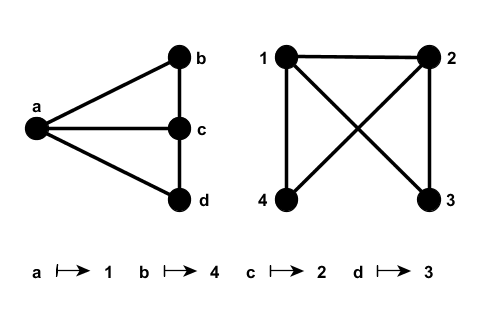
\includegraphics[width=\textwidth]{chapter1/fig/GI}
        \caption{Graph isomorphism}
        \label{fig:GI}
    \end{subfigure}
    ~
    \begin{subfigure}[b]{0.3\textwidth}
        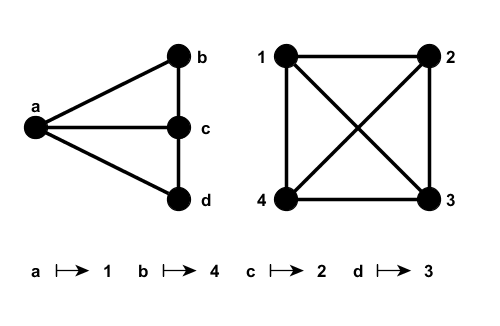
\includegraphics[width=\textwidth]{chapter1/fig/monomorphism}
        \caption{Graph monomorphism}
        \label{fig:monomorphism}
    \end{subfigure}
    ~
    \begin{subfigure}[b]{0.3\textwidth}
        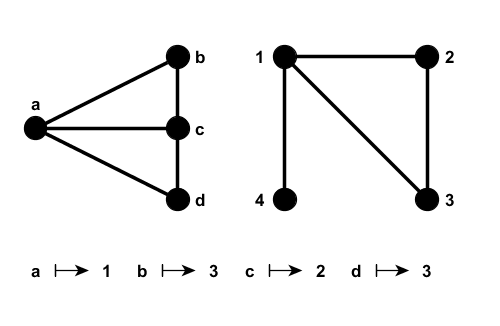
\includegraphics[width=\textwidth]{chapter1/fig/homomorphism}
        \caption{Graph homomorphism}
        \label{fig:homomorphism}
    \end{subfigure}
    \caption[Exact graph matching problems]{Exact graph matching problems}\label{fig:Exact_GM}
\end{figure}

%\subsection{Compexity}
All problems except graph isomorphism are proofed to be $NP-$complete~\cite{Garey_NPComplet}. This can be shown through a reduction of the respective matching problem to the clique problem. The graph isomorphism is currently shown to be $NP-$hard~\cite{Garey_NPComplet,Schoening_GI}. For some special types of graphs there exist however polynomial time algorithms (e.g. for %planar graphs~\cite{Hopcroft_Wong} and 
trees~\cite{Aho_Ullman, Garey_NPComplet}).

The exact graph matching problems are often too strict and intractable for the practical application and therefor do not lie in the focus of this work. In following we describe several approaches for to solving them.
% ---------------------------------------------------------------------------------------------------------------------------------
\section{Methods for solving exact graph matching problems}
The most used approach to solve an exact graph matching problem is based on a tree search with backtracking. This method starts with an empty set of correspondences and tries stepwise to expend it according to provided rules until a complete solution is found. Each partial solution represent a node of a search tree and all nested solutions build a branch in this tree. If it happens, that in some step a current set of correspondences cannot be expended further due to problem constraints, the current branch in the tree is cut. The method backtracks to the last feasible solution and tries to find another way to expend it further. The algorithms based on a tree search are very slow, if they need to traverse a whole tree. However, they can be speeded up by applying some heuristics to detect unpromising branches and exclude them from the search. The most known algorithm in this group, which uses depth-first-rule to traverse a tree, is the branch and bound algorithm~\cite{Reingold}.

The one of the first algorithms, that used the described technique, is the one by Ullman~\cite{Ullmann}. Later it was extended and improved mostly by the suggestion of a new pruning heuristics. A small comparison of different algorithms in this group with diverse heuristics is reported in~\cite{Lee2013}. We also want to mention here another well known algorithm on graphs, which uses the tree search method, namely the algorithm by Bron and Kerbosch~\cite{BronKerbosch} for finding cliques in an undirected graphs. The last problem closely related to the graph matching, as the maximal common subgraph problem can be reduced to the problem of finding the maximal clique~\ToDo{cite}.

From the other techniques we want to mention the algorithm described by MacKay~\cite{McKay}, which uses group theory to solve graph isomorphism problem, and an approach based on decision trees~\cite{Messmer1999,Shearer2001,Shearer1998} for matching graph ((sub)graph isomorphism) against a set of graphs.
% ---------------------------------------------------------------------------------------------------------------------------------
\section{Inexact graph matching}
As we mentioned above exact graph matching problems are often not applicable to real world problems. There are two possible reasons for that. On the one hand, that  natural variations in the structure of graphs, that describe a same object. Those variations could be a consequence of object deformations or noise influence, that can occur in some real word applications. On the other hand, solving a graph matching problem exactly can be time and/or memory consuming. As a consequence one can be interested in solving graph matching problem inexactly. In this case, no edge preserving mapping between the nodes of two graphs is required.

\vspace{-12pt}
\begin{figure}[htb]
	\centering
	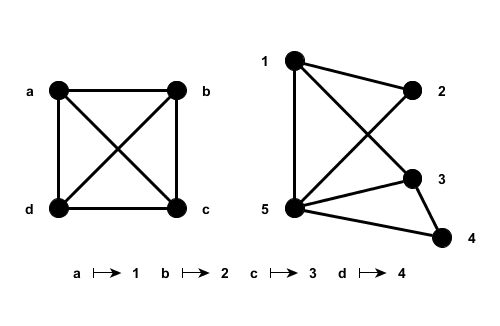
\includegraphics[width=0.5\textwidth]{chapter1/fig/inexactGM}
    \caption{Inexact graph matching}
    \label{fig:inexact_GM}
\end{figure}
\vspace{-10pt}
Let us recall the problem statement \eqref{gGMP}: 
\begin{equation*}
m = \argmax_{\hat{m}}S(G^I, G^J, \hat{m})
\end{equation*}
where $S(G^I, G^J, \hat{m})$ defines a similarity measure between the attributed graphs $G^I = (V^I, E^I,D^I)$ and $G^J = (V^J, E^J,D^J)$. The mapping $m$ is required to be total and sometimes also injective, to guarantee one-to-one matching.

Depending if an algorithm for solving \eqref{gGMP} finds a global solution or not, it is called \emph{optimal} or~\emph{suboptimal}. The choice, which algorithm to select depends on a specific problem. It should be noted, that optimal inexact algorithms is not necessary faster than the exact one. On the other hand, suboptimal inexact algorithms often do not have any performance guarantee.

There are also different ways to define a similarity function $S(G^I,G^J,m)$, which leads to high number of different approaches inside the group of inexact graph matching algorithms. In the following section we summarized the most common forms of the objective function of the problem~\eqref{gGMP}.
% ---------------------------------------------------------------------------------------------------------------------------------
\subsection{Graph matching objective function}
In some literature instead of defining a similarity function as in \eqref{gGMP} one speaks about dissimilarity between two graphs~\cite{Herault1990_SimulatedAnnealing,FastPFP,Lyzinski2015,Roth2001,Vogelstein_BrainGraphs,Zazlavskiy2008_PATH}. The goal in this case is to minimize it. Two formulations of the problem are however equivalent and one can easy transform one into other.
% ---------------------------------------------------------------------------------------------------------------------------------
\subsubsection{Quadratic Optimization Problem}
Let consider two attributed graphs $G^I = (V^I, E^I,D^I)$ and $G^J = (V^J, E^J,D^J)$. We want to find a mapping $m$ between the nodes of this graphs. Let the size of the graphs be $n_1$ and $n_2$ respectively. Generally, $n_1$ and $n_2$ can be different, but then we assume without losing generality $n_1\le n_2$. Here and further, we require a mapping $m$ in \eqref{gGMP} to be total and injective, which guarantees, that each node of the first graph will be matched to exactly one node of the second graph (one-to-one matching). 

We start first with a even stricter assumption, that $n_1=n_2=n$ and the matching is bijective. In this case a mapping between nodes of two graphs defines a permutation $\sigma$ of the set $\{1,\dots,n\}$. Each permutation $\sigma$ can be represented by the permutation matrix $P=\{P_{ij}\}$, where
\begin{equation*}
P_{ij}=\begin{cases}
 1, & \text{if } \sigma(i)=j, \\
 0, & \text{otherwise.} \\
\end{cases}
\end{equation*}
We denote with $\Pi_n$ the set of all feasible permutations:
\begin{equation*}
\Pi_n=\{P\in\{0,1\}^{n\times n}|\sum_{i=1,\dots,n}P_{ij}=\sum_{j=1,\dots,n}P_{ij}=1\quad\forall i,j=1,\dots,n\}
\end{equation*}
Let matrices $A^I$ and $A^J$ be the adjacency matrices of the graphs $G^I$ and $G^J$ respectively. We assume, that in case of weighed graphs, the adjacency matrices contain edge weights, instead of binary values. We can now formulate the graph matching problem as~(compare with \cite{Herault1990_SimulatedAnnealing,FastPFP,Lyzinski2015,Roth2001,Umeyam1988,Zazlavskiy2008_PATH}):
\begin{equation} \label{eq:QAP1}
%P = \argmin_{\hat{P}\in\Pi_n}\|A^I\hat{P}-\hat{P}A^J\|^2
P = \argmin_{\hat{P}\in\Pi_n}\|A^I-\hat{P}A^J\hat{P}^T\|^2+\|D^I-\hat{P}D^J\|^2
\end{equation}
where $\|\cdot\|$ is the matrix Frobenius norm. Some authors (e.g. Vogelstein et al. in~\cite{Vogelstein_BrainGraphs}) use slightly different, but equivalent reformulation of it, namely:
\begin{equation} \label{eq:QAP2}
P = \argmin_{\hat{P}\in\Pi_n}\|A^I\hat{P}-\hat{P}A^J\|^2+\|D^I-\hat{P}D^J\|^2,
\end{equation}
After some transformations, the problem \eqref{eq:QAP1} can be reformulated as~(see~\cite{Burkard98thequadratic}, Appendix~\ref{appendixA}):
\begin{equation} \label{eq:QAP3}
P = \argmin_{\hat{P}\in\Pi_n}vec(\hat{P})^T(-(A^J)^T\otimes(A^I)^T)vec(\hat{P})+\tr(D\hat{P}^T)
\end{equation}
where $\otimes$ denotes the Kronecker product and $vec(\hat{P})$ is a column-wise vectorization of $\hat{P}\in\Pi_n$.

The objective function of \eqref{eq:QAP3} is a negation of the objective of the \emph{quadratic assignment problem}% with linear cost matrix set to zero
, which is know to be $NP-$hard~\cite{Burkard98thequadratic,Sahni1974}.

The both formulations~\eqref{eq:QAP1},~\eqref{eq:QAP3} have their advantages and disadvantages. The main benefit of \eqref{eq:QAP1} is the low space complexity $\mathcal O(n^2)$, where the space requirement of \eqref{eq:QAP3} estimates with $\mathcal O(n^4)$. This makes the second formulation tractable only for relative small graphs. The drawback of both formulations is the strict penalization function of edge disagreements, namely the squared euclidean distance between matched edges. This follows straight forward from \eqref{eq:QAP1}. In this sense the last formulation can be easily generalized in the way, we represent below. 

We return back to the case where $n_1\not=n_2$. Let denote with a binary vector $x\in \{0,1\}^{n_1n_2}$ the column-wise vectorization of the assignment matrix $P$, which is not necessary a permutation matrix anymore. It is obviously, that $x_{(j-1)n_1+i}=1$, if a node $v_i\in V^I$ is matched to a node $u_j\in V^J$, and $x_{(j-1)n_1+i}=0$ otherwise. For simplicity we will write further $x_{ij}$ instead of complicated form $x_{(j-1)n_1+i}$.
 
%For this, we also assume, that $|V^I|=n_1$, $|V^J|=n_2$ and $n_1$ is not necessary equal to $n_2$. The maximum number of possible matches is though equal to $\min(n_1, n_2)$.

To measure a similarity between graphs one considers two different kinds of similarities: second-order \emph{edge similarity} and first-order \emph{node similarity}. The first one is defined as a function of the edges $s_E:E^I\times E^J\rightarrow\mathbb{R}$ and should penalize a disagreements in the structure of two graphs. The second one $s_V:V^I\times V^J\rightarrow\mathbb{R}$ represent additional constrains on the possible node correspondences.

%Now we want to reformulate the objective function in \eqref{gGMP} using introduced node and edge similarity functions.
%A found mapping m (see Eq.~\eqref{gGMP}) gives us a set of node correspondences, which maximizes the similarity value between two graphs. Such a subset can be represented by a binary vector $x\in \{0,1\}^{n_1n_2}$, where $x_{(j-1)n_1+i}=1$, if node $v_i\in V^I$ is matched to node $u_j\in V^J$, and $x_{(j-1)n_1+i}=0$ otherwise. For simplicity we will write further $x_{ij}$ instead of $x_{(j-1)n_1+i}$.
%\footnote{Vector $x$ is a column wise vectorization of the correspondence matrix $X\in\{0,1\}^{n_1\times n_2}$, where $X_{ij}=1$, if the node $v_i\in V^I$ is matched to the node $v_j\in V^J$, and $0$ otherwise.}

Using the introduced notation and definitions of the node and edge similarity functions the function $S(G^I,G^J,m)$ in~\eqref{gGMP} can be now rewrite as follows:
\begin{equation}\label{eq:sumQAP}
	S(G^I,G^J,m)=\sum_{\substack{x_{ij}=1\\x_{i'j'}=1}}s_E(e_{ii'},e_{jj'}) + \sum_{x_{ij}=1}s_V(v_{i},v_{j})
\end{equation}
This formula can be also expressed in matrix form. We define an \emph{affinity} or \emph{similarity matrix} $S\in\mathbb{R}^{n_1n_2\times n_1n_2}$, whose diagonal elements are $s_V(v_i, u_j)$ and non-diagonal elements are $s_E(e_{ii\prime}, e_{jj\prime})$. Using this matrix we become the following formulation of the graph matching problem as an quadratic optimization problem \cite{Cho2014_Haystack, Cho2010_RRWM, Cho2012_ProgressiveGM, Conte2004,Rangarajan1996_GAGM,Leordeanu2005_SM,Leordeanu2009_IPFP}:
\begin{alignat}{2}
    &     && \argmax_x{x^TSx}                           \label{eq:gQAP1}\\ %\notag\\
    & \text{s.t. } &&  x\in \{0,1\}^{n_1n_2}            \label{eq:gQAP2}\\
    &             &&  \sum_{i=1\dots n_1} x_{ij}\le 1    \label{eq:gQAP3}\\
    &             &&  \sum_{j=1\dots n_2} x_{ij}\le 1    \label{eq:gQAP4}
\end{alignat}
We notice, that in the case, where $n_1=n_2$, both conditions (\ref{eq:gQAP3}) and (\ref{eq:gQAP4}) will be fulfilled with equality. We call this constraints~\emph{two-way constrains}, as the enforce one-to-one matching .

One can easily see, that the formulation \eqref{eq:QAP3} can be obtained from \eqref{eq:QAP1}-\eqref{eq:gQAP4} by setting $S=-(A^J)^T\otimes(A^I)^T$.
%A Quadratic Optimization Problem is known to be \emph{NP}-hard \cite{Sahni1974}. This limits greatly the size of a graph, for which a exact solution can be calculated in reasonable time. Due to this there are a number of algorithms \cite{Cho2014_Haystack, Cho2010_RRWM, Cho2012_ProgressiveGM, Chui2003, Suh_CVPR2015}, that solve graph matching problem inexact.

Below we list a different ways to define a node and edge similarities between two attributed graphs we found in the literature.

%\subsubsection{Edge similarity}
\textbf{Edge similarity}

One possible approach to calculate an edge similarity is to calculate \emph{edge dissimilarity} $d_E:E^I\times E^J\rightarrow\mathbb{R}$ first and then transform it into similarity by using, for example, one of the following functions~\cite{Cho2014_Haystack, Cho2009_AgglClustering, Cho2010_RRWM,Cho2012_ProgressiveGM}:
\begin{itemize}
	\item $s_E(e_{ii\prime}, e_{jj\prime})= exp(-\frac{d_E(e_{ii\prime}, e_{jj\prime})^2}{\sigma^2_{s}})$
	\item $s_E(e_{ii\prime}, e_{jj\prime})= \max(\beta - d_E(e_{ii\prime}, e_{jj\prime})/\sigma^2_{s},0)$
\end{itemize}
where $e_{ii\prime}\in E^I$ and $e_{jj\prime}\in E^J$. The parameters $\sigma_s$ and $\beta$ define a sensibility of a graph matching algorithm to the dissimilarities between the graphs.

This leads us to the question how to calculate edge dissimilarity. The most obvious way is to compare a weights of the edges, if such are provided. An other alternative could be to use length of the edges~\cite{Cho2014_Haystack, Cho2009_AgglClustering, Cho2010_RRWM,Cho2012_ProgressiveGM}, if coordinates of the nodes in some system (usually, Cartesian coordinates) are known. It a significant assumptions, which holds however for almost all graphs arose in practical application.

Sometime a node attributes can be used to calculate edge dissimilarities. For example, if graph nodes are described by an ellipse with known center coordinates and orientation one can calculate so-called geometric dissimilarity of the edges~\cite{Cho2009_AgglClustering,Cho2012_ProgressiveGM}:
\begin{alignat}{4}\label{eq:geomDiss}
& d(e_{ij},e_{i'j'}) && =\frac{1}{2}(d_{geo}(m_j|m_i) && +d_{geo}(m_i|m_j)) \\
& d_{geo}(m_j|m_i) && =\frac{1}{2}(\|x_{j'}-H_{i}x_j\| && + \|x_{j}-H^{-1}_ix_{j'}\|) \\
& d_{geo}(m_i|m_j) && =\frac{1}{2}(\|x_{i'}-H_{j}x_i\| && + \|x_{i}-H^{-1}_{j}x_{i'}\|) 
\end{alignat}
where $m_i$ is a correspondence between nodes $v_i$ and $v_{i'}$ and $H_i$ is an affine homography from $v_i$ to $v_{i'}$ estimated based on elliptic regions around each node.

An another way to calculate edge similarities could be to use directly some similarity measure, such as cosine similarity.

\textbf{Node similarity}

%\subsubsection{Node similarity}
If a given graphs have node attributes, the most direct method to measure a similarity of two nodes is to compare their attributes. In the most of the seen literature, the node attributes are represented by a $k-$dimensional real vectors: $D^i,D^J\subset\mathbb{R}^k$. This means, we can adopt all techniques\footnote{with except of the geometric dissimilarity measure} described in previous paragraph to define a node similarity function. Additionally, in case when node attributes can be considered as some distribution (e.g. distribution of gray values of an image around a node), one can think to use metrics to measure distance between two distributions. For example, Schellewald and Schn\"orr~\cite{Schellewald2005} used the earth mover distance for this propose.
% ---------------------------------------------------------------------------------------------------------------------------------
\subsubsection{Error correcting graph matching}
Another way to measure the similarity between two graphs is based on a \emph{graph edit distance}~\cite{Bunke1983_inexactGM}. The graph edit distance is defined through costs of \emph{graph edit operations}, that transform on graph into another. Those operations are insertion, deletion and substitution of nodes and edges of a graph. An algorithm, that uses graph edit distance for graph matching, is often called~\emph{error correcting}~\cite{Conte2004}.

Consider two attributed graphs $G^I = (V^I, E^I,D^I)$ and $G^J = (V^J, E^J,D^J)$ and matching $m$ between subsets $\bar{V}^I,\bar{V}^J$ of $V^I$ and $V^J$ respectively. The edit operations on nodes can be directly defined by the mapping $m$~\cite{Bunke1998_ErrTolerantGM}:
\begin{itemize}
	\item if $m(v_i)=v_j$ for $v_i\in\bar{V}^I,v_j\in\bar{V}^J$, then a node $v_i$ is \emph{substituted} by a node $v_j$
	\item nodes in $V^I\backslash\bar{V}^I$ are \emph{deleted}
	\item nodes in $V^J\backslash\bar{V}^J$ are \emph{inserted}.
\end{itemize}
An edit operation of an edge is defined based on a transformations applied to it's end nodes. For example, insertion of a node $v_j\in V^J$ implies that all edges, connected to this node, are also inserted. Alternatively, if a node $v_i\in V^I$ is deleted, then all edges incident to this node are also deleted. We say, that an edge $\{v_i,v_{i'}\}\in E^I$ was substituted by an edge $\{v_j,v_{j'}\}\in E^J$, if the nodes $v_i,v_{i'}$ were mapped in $v_j,v_{j'}$.

We assume, that all operations can be performed simultaneously. Let $S=\{s_1,s_2,\dots,\newline s_k\}$ denote a set of operations needed to transform the graph $G^I$ into the graph $G^J$. 
Each edit operation $s_i, 1\le i\le k,$ has an assigned nonnegative cost $c(s_i)$. The cost of the whole sequence $S$ is defined then as $\sum_{i=1}^{k}c(s_i)$. Using this we define a \emph{edit distance} between the graphs $G^I$ and $G^J$ as follows~\cite{Bunke1983_inexactGM, Wang1995}:
\begin{eqnarray} \label{eq:editDist}
dist(G^I,G^J,m) = \min\limits_{S=\{s_1,\dots,s_k\}}c(S)
\end{eqnarray}
The task of the error-corrected graph matching is to find such a mapping $m$ between $V^I$ and $V^J$, which induces a cheapest transformation between the graphs.

The cost functions of each operation are often defined as a functions of edge weights and node attributes. Their exact definitions depend however on a specific application. Sometimes, it can be helpful, when the distance measure~\eqref{eq:editDist} defines a metric, which is not automatically the case. Bunke and Allermann~\cite{Bunke1983_inexactGM} have shown that, the graph edit distance can fulfill the properties of a metric under a specific conditions on the cost functions of the individual edit operations. For example, one if this conditions is, that a single operation is always preferred to a sequence of two operations with the same result (triangular inequality of the operation cost functions). Later, Bunke and Shearer~\cite{Bunke1998_graphDist} suggest a new graph edit distance, that is not depending on the cost of the edit operations, and is a metric.

An interesting question is, how does the error corrected graph matching problem correspond to the other matching problems defined previously. It was shown in~\cite{Bunke1999_UnderlyingCosts}, that graph isomorphism, subgraph isomorphism and maximum common subgraph problems can be considered as a special cases of the error correcting graph matching. The same holds for the inexact graph matching problem formulated as in~\eqref{eq:QAP1}. This is easy to see, if one rewrite the objective function of ~\eqref{eq:QAP1} as $\sum_{i=1}^n\sum_{j=1}^{n}(A^I_{ii'}-A^J_{\sigma(i)\sigma(i')})^2$. Comparison of this expression with the definition of $c(S)$ in~\eqref{eq:editDist} leads us direct to the idea, how to set the edge insertion/deletion/substitution cost functions, to make the problem formulations equivalent: 
\begin{equation*}
c(e_{\text{subst}})=(A^I_{ii'}-A^J_{\sigma(i)\sigma(i')})^2\quad c(e_{\text{insert}})=(A^J_{\sigma(i)\sigma(i')})^2\quad c(e_{\text{del}})=(A^I_{ii'})^2
\end{equation*}
% ---------------------------------------------------------------------------------------------------------------------------------
\section{Methods for solving inexact graph matching problems}
In following we briefly describe a common approaches for solving inexact graph matching problems in field of Computer Vision and Pattern Recognition. We subdivided them into groups based on their main idea.
% ---------------------------------------------------------------------------------------------------------------------------------
\subsection{Discrete optimization}
\subsubsection{Tree search methods}
Similar to the exact graph matching problems a tree based methods with backtracking were successfully applied to solve inexact matching problems. They were especially wild used for the error-correcting graph matching. In this case a searching procedure can be efficiently guided, so that the required time is shorter than exponential time, which is needed by a blind searching. This can be done by defining the score of the tree nodes as a sum of two scores: a matching score of a current partial solution and a heuristically estimated score of a remaining nodes. The algorithms in this group differ mainly in a suggested heuristics for calculation of future costs and in a rules, for tree traversing. The most used strategies for tree traversing are depth-first-search~\cite{Cormen} and $A^*$-Algorithm~\cite{AStar}.

One of the first algorithms for inexact graph matching based on the three search was presented by Tsai and Fu in~\cite{Fu1979}. It is an optimal inexact graph matching algorithm. For further examples of the three search methods for inexact graph matching we refer to \cite{Bunke1983_inexactGM,Shapiro1981,Wang1995}.
\subsubsection{Simulated Annealing}
Simulated annealing is a heuristic for searching the global optimum of a given energy function~\cite{Burkard98thequadratic}. It is an extension of the Metropolis Algorithm~\cite{Metropolis}, that was suggested for finding an equilibrium of a physical system consisting of individual particles by heating it first and then cooling it slowly down. Speaking in terms of a graph matching problem, its solutions define states of a system and corresponding objective scores it's energy. The idea is to find a state with the lowest energy by performing some random changes in a system. This can be a random exchange of correspondences between two pairs of matched nodes. A change, that increases the total dissimilarity of graphs, is always accepted. On the other side, a change, that increases energy function, is accepted with some probability. This probability and number of changes per iteration is controlled by the temperature parameter $T$. The bigger $T$ the viewer changes are allowed and the smaller the accepted probability is. 

The application of the simulated annealing to the graph matching problems can be found in~\cite{Herault1990_SimulatedAnnealing}. This heuristic can also be used to solve a quadratic assignment problem~\cite{Burkard98thequadratic}.
% ---------------------------------------------------------------------------------------------------------------------------------
\subsection{Continuous optimization}
This group of methods is one of the biggest and deep investigated. The main idea is to transform the inexact graph matching problem into a continuous optimization problem. This can be done, for example by relaxing the integer constraints in the discrete optimization problems~\eqref{eq:QAP1},~\eqref{eq:gQAP1}. A found solution must be converted afterwards back in the discrete domain. Depending on techniques, applied to solve a continuous problem, we subdivide this group into several subgroups. The list of the algorithms, presented here, is not complete. As we already mentioned, we selected mainly the classical approaches and/or those, we investigated during the work on this thesis.

The first subgroup of the algorithms contains the algorithms, that relax all constraints of a graph matching problem, find a continuous solution of the new nonlinear problem and project it back into discrete domain. 

In 1996 Gold and Rangarajan presented a graduated assignment algorithm for graph matching (GAGM)~\cite{Rangarajan1996_GAGM}. It is an iterative algorithm, which uses \emph{deterministic annealing}\footnote{Deterministic annealing is similar to the simulated annealing, but uses deterministic techniques to find a minimum of an energy function by a current value of a temperature parameter~\cite{Rose1991_DA}.} to solve the graph matching problem formulated as~\eqref{eq:gQAP1}. The authors use Taylor series approximation to relax the initial quadratic assignment problem to linear assignment problem. The two-way constrains are enforced at each iteration by converting a  found continuous solution into a double stochastic matrix by applying exponentiation and Sinkhorn normalization~\cite{Sinkhorn1964}. This technique is called \emph{soft-assign}. The deterministic annealing was also used in~\cite{Rangarajan96_LagRelax} to solver Lagrangian Relaxation of the problem~\eqref{eq:QAP1} and in the robust point matching algorithm with thin-plane spline (RPM-TPS)~\cite{Chui2003}. The solution, obtained by this method is however not necessary optimal and the behavior of the algorithms depends highly on the selected parameters, especially those, which control the annealing schema.

Another iterative algorithm was proposed in~\cite{Leordeanu2009_IPFP} and is called an integer projected fixed point method (IPFP). It consists of two steps, which we shortly describe below. In the first step, an initial solution has to be chosen. It can be, for example, a continuous or discrete solution obtained by some other algorithm. The second step iteratively improves this solution by applying \emph{Frank-Wolfe algorithm}~\cite{Wolfe1956} adapted to the graph matching problem. This algorithm finds first the best search direction by solving an linear assignment problem. The last arises as in GAGM by the maximization the first-order Tailor series approximation of the objective function. The maximization is performed in the discrete domain using the Hungarian algorithm~\cite{Kuhn1955}. Then the initial objective function is further maximized in a continuous domain along found direction. The authors show, that in the praxis IPFP tens to converge towards discrete solutions, that are close to the optimum.

The Fast Approximative Quadratic Programming Algorithm (FAQ), presented in~\cite{Vogelstein_BrainGraphs}, also uses Frank-Wolfe algorithm to solve a continuous relaxation of the problem~\eqref{eq:QAP2}. However FAQ perform completely in a continuous domain and has the third step, which maps a found continuous solution back onto discrete domain. Unlike IPFP, the FAQ algorithm do not use the similarity matrix $S$. This gives it a big advantage of the less space requirement, which make it possibly to apply the algorithm to graphs of a big size\footnote{Evaluation results in the paper include test with a graphs with up to $1000$ nodes}. 

Another approach, that uses Frank-Wolfe algorithm, is the PATH-Algorithm~\cite{Zaslavskiy2010}. The algorithms finds first the global optimum of the Lagrangian relaxation of the problem~\eqref{eq:QAP2}. For this the Newton method~\cite{Book_ConvOpt} is used. Afterwards the found solution is projected back onto discrete domain by solving a sequence of convex and conclave problems, which are solved Frank-Wolfe algorithm.

Very close to~ IPFP is the fast projected fixed-point algorithm (FastPFP) proposed by Lu et al.~\cite{FastPFP}, that uses \emph{projected fix point method} to find a solution of a continuous relaxation of the problem~\eqref{eq:QAP1}. Compared to IPFP the new algorithm uses projections onto a continuous domain, instead of discrete. Furthermore, the authors proofed the linear convergence rate of their algorithm, whereby the convergence rate of IPFP is unknown. The FastPFP, similar to FAQ, do not have a memory issues because it does not use a similarity matrix $S$ and is generally faster than both IPFP and FAQ, because it does not solve a linear assignment problem on each iteration.

A completely different approach to solve graph matching problem was suggested by Schellewald and Schn\"orr~\cite{Schellewald2005}. They formulated graph matching problem as a regularized bipartite matching problem~\cite{Diestel2000}, which is then relaxed to a convex semidefinite program. The last can be solved with standard algorithms, such as the interior point method~\cite{Book_ConvOpt}. A novelty of the algorithm consists in a probabilistic post-processing step, which convert a found continuous solution  into discrete one. The suggested algorithm is easy to apply, as it has only one parameter. However the considered relaxation problem has a squared size comparing to initial problem~\cite{Cour2006}. Consequently, the algorithm is not suitable for big graphs.
% ---------------------------------------------------------------------------------------------------------------------------------
\subsubsection{Spectral methods}
A big group of algorithms for solving graph matching problems is built by those, which use an eigenvalue decomposition~\cite{Book_ConvOpt} of the adjacency matrices of given graphs. The idea behind this is, that the eigenvalues and eigenvector of the adjacency matrices of two isomorphic graphs are equal, because they are invariant to the node permutation.\ToDo{cite}

One of the first algorithms, which uses spectral techniques, is the one by Umeyama\newline~\cite{Umeyam1988}. He considers the case, when two graphs have the same number of nodes and matching between them is bijective. This means, that a desired correspondence matrix must be a permutation matrix. The author proofs, that an orthogonal matrix, which minimizes the objective function of~\eqref{eq:QAP1}, can be formulated based on the eigenvalue decomposition of the adjacency matrices of given graphs. The terms of this formulation are used to define a linear assignment problem, whose solution is a solution of the initial problem. In case, when given graphs are sufficiently close, those solution is optimal or nearly optimal.

We notice, that this algorithm is highly limited in it's application due to its requirements. We also want to mention, that it works only with graph geometry and does not consider attributes of nodes and edges.

The more resent algorithm is this group of methods is called spectral matching (SM)~\cite{Leordeanu2005_SM}. The algorithm works with the general formulation~\eqref{eq:gQAP1}. It relaxes both two-way and integer constrains~\eqref{eq:gQAP2}-\eqref{eq:gQAP4} and obtain the optimal solution of this relaxation by taken the principal eigenvector of the matrix $S$. This is done by using \emph{the power iteration method}~\cite{PowerIteration}. The found continuous solution is binarized by applying a simple greedy heuristic, that enforces previously relaxed matching constrains.

A generalization of the SM algorithm is proposed in~\cite{Duchenne2011}. The authors suggest to consider similarities between tuples of nodes and not only pairs to improve graph matching quality. They formulate a new problem using hyper-graphs and tensor notation. The solution strategy is however the same, as in~\cite{Leordeanu2005_SM}: the solution is approximated with the principal eigenvector of the matrix $S$ and discretized afterwards. However, the power iteration method should be adopted to the tensor based problem, as it cannot be applied directly.

Before going to the next section we want shortly describe a max-pooling approach by Cho and Duchenne~\cite{Cho2014_Haystack}, which uses ideas similar to both GAGM~\cite{Rangarajan1996_GAGM} and SM~\cite{Leordeanu2005_SM}, but replaces one of the sum in a updating step with maximum-operation. The algorithm solves the graph matching problem formulation~\eqref{eq:gQAP1} by relaxing its integer constraints and omitting sum constraints. To approximate a solution of $\argmax_{x}x^TSx$ the max-pooling algorithm similar to GAGM uses first order Taylor expansion of the objective function. The maximization of the Taylor approximation can be done by the power method as it is done in SM.
The resulting update formula of the correspondence $(v_i,v_j),v_i\in V^I,v_j\in V^J$ has the form:
\begin{equation}
(Ax)_{ij}=x_{ij}s_V(v_i,v_{j})+\sum_{i'\in N_i}\sum_{j'\in N_j}x_{i'j'}s_E(e_{ii'},e_{jj'}),
\end{equation}
where $N_i$ denotes a direct neighborhood of a node $v_i$, i.e. set of its adjacent nodes.
The max-poling algorithm uses a maximum function instead of the second sum in the second term, which leads to
\begin{equation}
(Ax)_{ij}=x_{ij}s_V(v_i,v_{j})+\sum_{i'\in N_i}\max_{j'\in N_j}x_{i'j'}s_E(e_{ii'},e_{jj'}).
\end{equation}
This simple idea helps to suppress a noisy entries of the outlier matches, because the last have more likely low similarity values. The proposed algorithm shows very good results in presents of numerous outliers, although there is no theoretical justification of its convergence.
% ---------------------------------------------------------------------------------------------------------------------------------
\subsubsection{Probabilistic frameworks}
Another group of algorithms applies \emph{relaxation labeling} to solve graph matching problem. The aim of the relaxation labeling is to find an optimal assignment between set of labels and set of objects. Each label has some initial probability to be assign to certain object. Those probabilities are set based on some informations known about the objects. In terms of graph matching problem, nodes of a one graph are considered as objects and nodes of another graph as labels. Initial probabilities of assignments between the nodes are calculated  based on the node and edge attributes. 

The earlier works on this formulation are the one by Fischer and Elschlager~\cite{Fischler1973} and Rosenfeld et al.~\cite{Rosenfeld1976}. In both cases, proposed algorithms start with some initial label probabilities and try to reduce a labeling ambiguities at each iteration based on labels of neighboring nodes. The process runs till convergence or some predefined number of iterations. The algorithms are heuristic, but reduce the complexity of the initial problem to polynomial~\cite{Christmas1995}.

A first algorithm with theoretically proofed update rule is suggested by Kittler and Handcock~\cite{Hancock_Kittler}. This was later improved by Christmas at al.~\cite{Christmas1995}, who suggested a method to included provided node attributes and edge weights into update rule of the labeling probabilities and not only in the initialization step.

Later algorithms formulate graph matching problem as Maximum A Posteriori probability~(MAP) estimation. For example the matching process in~\cite{Hancock_StrucMatch} is a process of node exclusion and insertion, so that MAP rate monotonically increases in each iteration. This technique is suggested to effectively cope with the possible outliers in the sets of graph nodes. A node is considered as an outlier, if its deletion improves the consistency in the structure of two graphs. The structural constrains hereby are defined by a dictionary of feasible mappings between local neighborhoods (super-cliques) of nodes of two graphs. The algorithm shows good results in case of big number of outliers, is however slow.

Another interesting idea is presented in~\cite{Hancock_EM_SVD}. Given two graphs, nodes of the first graph are considered as an observed data and the nodes of the other as hidden random variables. In this formulation the graph matching problem is solved using~\emph{Expectation-Maximization algorithm} (EM)~\cite{EM_Dempster1977}. A similar algorithm is presented in the resent paper~\cite{Sanrom2012}. However, it works with the continuous correspondences between the graph nodes and projects them in the discrete domain using soft-assign technique described previously. It also includes structural information\footnote{Structural relations between nodes are given through adjacency matrix of a graph. Geometrical relations are represented as relative position of the nodes with respect to each other~\cite{Sanrom2012}.} into matching process, whereby the algorithm from~\cite{Hancock_EM_SVD} uses only geometrical information. Both algorithm are however not applicable to a big graphs due to unlimited increasing of the formulated density function with the size of a graphs~\cite{Armiti2014}. A new scalable graph matching algorithm, which also uses EM to solve the problem formulated in a maximum likelihood estimation framework, is presented recently in~\cite{Armiti2014}. The scalability is achieved there by including information about already known correspondence into calculation of the density function.
% ---------------------------------------------------------------------------------------------------------------------------------
\subsubsection{Methods using clustering techniques}
We want to emphasize independently the methods, that use clustering techniques to improve the graph matching score or performance.

Minsu Cho in~\cite{Cho2009_AgglClustering} proposes to use \emph{agglomerative clustering} on a set of candidate matches to effectively cop with outliers. The problem is formulates as in~\eqref{eq:gQAP1}. The considered graphs are attributed, so that candidate matches are selected based on the distance between node attributes. The algorithm is controlled by the dissimilarity measure between two clusters, which is defined as the average of $k$ smallest pairwise dissimilarities between points in two clusters. This linkage model is called by the authors \emph{adaptive partial linkage model}. Notice, that the points in clusters are pairwise correspondences between graph nodes. The dissimilarity between two nodes is defined as a linear combination of the node attribute dissimilarities and 
geometric dissimilarities defined as~\eqref{eq:geomDiss}. Empirical results show, that correct correspondences tend to build bigger clusters. In contrast to that, the outliers are likely to stay in small groups, so it possible to threshold them base on the cluster size.

Another algorithm based on the hierarchical clustering is suggested by Carcassoni and Hancock~\cite{Hancock_ModalClusters}. Its propose is to provide additional constraints, that can be used to improve the robustness of a graph matching algorithm against graph deformations. This was successfully achieved by using spectral methods to build the clusters. The $S$ eigenvectors associated with the first $S$ largest eigenvalues are selected as a cluster centers. After performing the clustering, a probabilistic matching algorithm is applied to match first the clusters and then the nodes inside the clusters.

Further benefit of using clustering methods in the potential complexity reduction. 
The first idea to achieve this is based on a hierarchical graph matching and appears for example in the work by Qui and Handcock~\cite{Hancock_GM_SpectralPart}. They suggest to use graph partition to create a new simplified graph, whose nodes represent clusters of initial graph. After partitioning graphs are matched in a similar manner as it is suggested by Carcassoni and Hancock~\cite{Hancock_ModalClusters}, where the derived clusters tie matching constraints. The used partition method is based on a spectral method and creates a set of non-overlapping node neighborhoods\footnote{A node neighborhood is defined here as a node with all its adjacent nodes.}. To build those they use Fiedler vector (eigenvector associated with the second smallest eigenvalue of a graph Laplacian matrix, see~\cite{Fiedler1975}). The authors provide a study, which shows, that the matching with proposed partition technique is stable under structural errors. Additionally, they show, that the simplified graphs preserve structure of initial graphs. The last was shown by performing clustering of a group of different graphs before and after simplification.

The second idea to reduce complexity of the initial matching problem uses graph clustering to create a set of independent subproblems. The matching is then performed for each subproblem independently and due to reduced problem size faster. A solution of the whole problem is then obtained by combining local solutions. The great benefit of such approach is the ability to parallelize the computation process, which can lead to the significant time reduction.

The described ides is followed by Lyzinski et al. in their resent paper~\cite{Lyzinski2015}. The aim of the authors is to parallelize a graph matching algorithm for matching very big graphs. However the problem, they consider, is semi supervised, meaning that correct correspondences between some nodes are known. It is obvious, that the matching results of the subdivided problem depends highly on the quality of the graph clusters and established correspondences between the clusters of two graphs. In a perfect clustering, node that should be matched, must lie in the corresponding subgraphs. To ensure that the clustering is sufficiently good, the authors propose a technique, that first spectrally embeds graphs and then jointly cluster them. The algorithm was successfully applied to the graphs with $20000-30000$ nodes.

%\subsubsection{Resent algorithms for big graphs}
% ---------------------------------------------------------------------------------------------------------------------------------
\section{Graph matching algorithms studied in this thesis}
In this section we want for completeness described detailed graph matching algorithm used in our framework for graph matching. However, we do not provide theoretical justification of the algorithm steps and refer a reader to the original paper for that. We use the notation introduced at the beginning of this chapter.

\subsection{Reweighted random walks for graph matching (RRWM)}
The presented here algorithm is designed by Minsu Cho et al.~\cite{Cho2010_RRWM} and interprets the graph matching problem~\eqref{eq:gQAP1}:
\begin{alignat*}{2}
    &     && \argmax_x{x^TSx}                           \tag{\ref{eq:gQAP1}}\\
    & \text{s.t. } &&  x\in \{0,1\}^{n_1n_2}            \tag{\ref{eq:gQAP2}}\\
    &             &&  \sum_{i=1\dots n_1} x_{ij}\le 1   \tag{\ref{eq:gQAP3}}\\
    &             &&  \sum_{j=1\dots n_2} x_{ij}\le 1   \tag{\ref{eq:gQAP4}}
\end{alignat*}
between two graphs $G^I=(V^I,E^I,D^I)$, $G^I=(V^I,E^I,D^I)$ in a random walk view. For this the authors define an association graph $G^{rw}=(V^{rw},E^{rw},D^{rw})$ based on the affinity matrix $S$. The set of nodes $V^{rw}$ of the new graph is represented by all possible correspondences between nodes in $V^I$ and $V^J$. This means, that $|V^{rw}|=n_1n_2$, where $|V^I|=n_1$ and $|V^J|=n_2$. We refer to a node of the graph $G^{rw}$ as $v_{ij}$ if it represent a correspondence pair $(v_i,v_j)$, $v_i\in V^I,v_j\in V^J$. The entry $S_{ij,i'j'}$ of the matrix $S$ defines the weight of the edge $\{v_{ij},v_{i'j'}\}\in E^{rw}$. We denote the weighted adjacency matrix of the graph $G^{rm}$ as $W$. An example of the construction is illustrated on the figure below. Note, that we omitted contradiction edges, whose weights are equal zero, e.g. $\{a1,b1\}$.

%\vspace{-30pt}
\begin{figure}[h] %\label{fig:RRWM} 
	\centering
    \begin{subfigure}[b]{0.33\textwidth}
        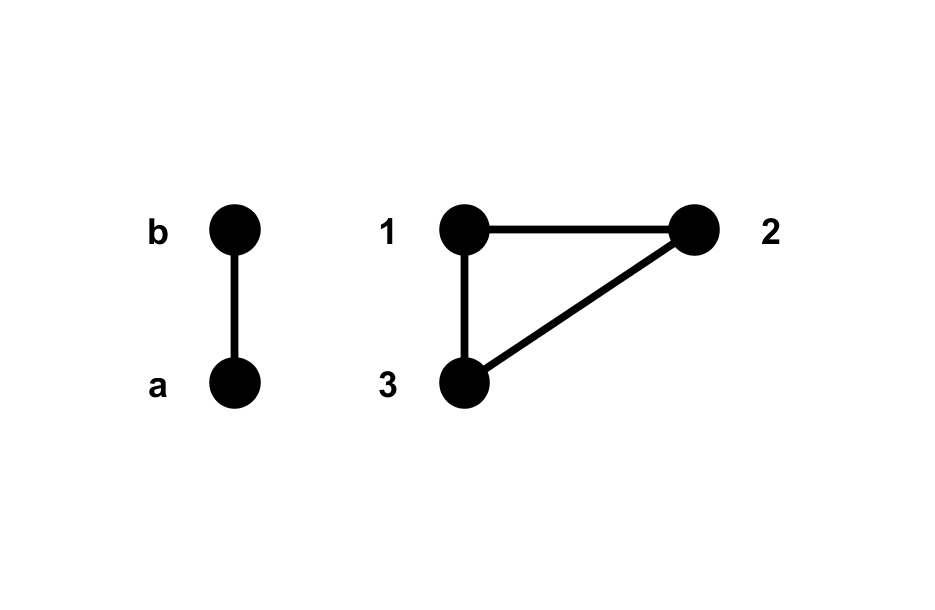
\includegraphics[width=\textwidth]{chapter1/fig/RRWM1}
        \caption{Two graphs to match}
        \label{fig:RRWM1} 
    \end{subfigure}
    ~
    \begin{subfigure}[b]{0.33\textwidth}
        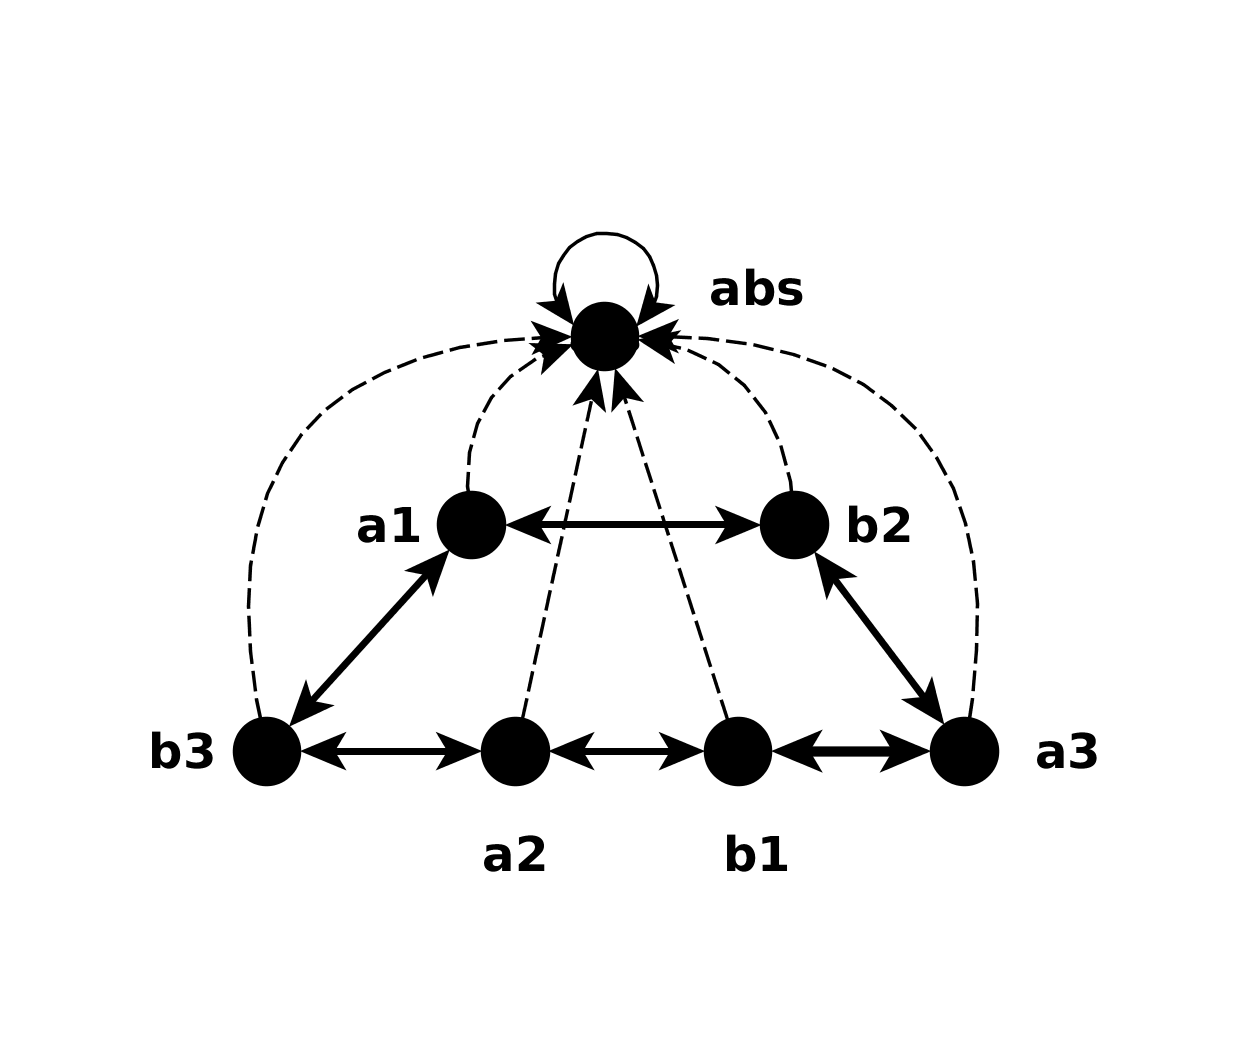
\includegraphics[width=\textwidth]{chapter1/fig/RRWM2}
        \caption{Association graph}
        \label{fig:RRWM2} 
    \end{subfigure}   
\caption{Association Graph of two given graphs for Reweighted Random Walk Method (compare to~\cite{Cho2010_RRWM})}
\end{figure}
%\vspace{-10pt}
It is obvious, that the graph matching problem between two graphs $G^I$ and $G^J$ is equivalent to finding a subset of nodes in the associated graph $G^{rw}$, so that the respective node correspondences between $V^I$ and $V^J$ satisfy matching criteria of the initial problem.
For finding such a subset the authors adopt the page ranking algorithm based on a random work, which is assumed to be a Markov chain~\cite{PageRank}. To describe a Markov chain one defines a transition matrix $P$. An usual approach to define a transaction matrix of a wighted graph $G^{rw}$ is to convert the weighted adjacency matrix $W$ of the graph into a stochastic matrix by the following normalization $P=D^{-1}W$, where $D$ is a diagonal matrix with entries $D_{kk}=\sum_{l}{W_{kl}}$. This method was, for example, used in PageRank algorithm~\cite{PageRank}. It is however not suitable for the graph matching proposes, as it treats false correspondences equal to all other correspondences. To avoid this problem Cho et al. introduce an additional absorbing node $v_{abs}$~(see Fig.~\ref{fig:RRWM2}) in the Graph $G^{rw}$, which represent a state, that can be reached from each node $v_k=v_{ij}\in V^{rw}$ with the probability $1-D_{kk}/D_{\text{max}}, D_{\text{max}}=max_{k}D_{kk}$, but can not be left any more. Using $D_\text{max}$ the matrix $W$ is converted into a stochastic matrix by its multiplication with the factor $1/D_{\text{max}}$.
Summarizing, the transition matrix $P\in\mathbb{R}^{(n_1n_2+1)\times(n_1n_2+1)}$ is defined as 
\begin{equation}P=
\begin{pmatrix}
	W/D_{\text{max}} & \mathbf{1}-d/D_{\text{max}} \\
	0\dots 0 & 1
\end{pmatrix} \label{eq:RRW_P}
\end{equation}
and update formula of the probability distribution of the Markov chain as
\begin{equation}\label{eq:RRW_MC}
\left(x^{(n+1)T},\ x_{\text{abs}}^{(n+1)}\right)=\alpha\left(x^{(n)T},\ x_{\text{abs}}^{(n)}\right)P+(1-\alpha)r^T,
\end{equation}
where $\mathbf{1}$ in~\eqref{eq:RRW_P} denotes a vector of size $\mathbb{R}^{n_1n_2\times 1}$ with all entries equal to $1$, $d=(D_{11},\dots,D_{n_1n_2})$ is the diagonal of the matrix $D$, $\alpha$ is a weighted factor and $r\in\mathbb{R}^{n_1n_2+1}$ is \emph{reweighted jump vector}.

A Markov chain, defined by Eq.~\ref{eq:RRW_MC} without second term, is denoted as an \emph{affinity-preserving random walk}. The distribution $\mathbf{\bar{x}}$ of unabsorbed random walks at time $n$ is defined as follows:
\begin{equation}\label{eq:RRWM_x}
\mathbf{\bar{x}}^{(n)}_{ij}=P(X^{(n)}=v_{ij}|X^{(n)}\not=v_{\text{abs}})=\frac{x^{(n)}_{ij}}{1-x^{(n)}_{\text{abs}}}, 
\end{equation}

where $X^{(n)}$ is a current location of a random walker at time $n$. The authors call $\mathbf{\bar{x}}$ a \emph{quasi-stationary distribution} of the absorbed Markov chain. They proof, that the distribution $\mathbf{\bar{x}}$ is proportional to the left principal eigenvector of $W$ and can be efficiently computed with power iteration method~\cite{PowerIteration}.

The second summand in the Eq.~\ref{eq:RRW_MC} represents the possibility of a random walker to make a jump with probability $(1-\alpha)$ into some constrained node, instead of following the edge. This term was proposed by the authors based on personalization approach for web pages ranking~\cite{Langville2003} as a way to include the matching constraints~\eqref{eq:gQAP3},~\eqref{eq:gQAP4} into random walk. The authors are pointing out, that without this term the matching constrains are incorporated only in the last discretization step of the algorithm, which leads to a weak local maximum. 

A procedure of generation the jump vector $r$ from a current quasi-stationary distribution $\mathbf{\bar{x}}$ consists of two steps. In the first step (\emph{inflation}) unreliable correspondences (i.e. small values in the vector $\mathbf{\bar{x}}$) are damped and the good correspondences are at the same time boosted. The second step (\emph{bistochastic normalization}) forces the matching constraints by transforming the matrix form of $\mathbf{\bar{x}}$ into double stochastic matrix using the normalization scheme of Sinkhorn~\cite{Sinkhorn1964}. 

\begin{algorithm}[h] 
	\KwIn{ weight matrix $W$, the reweight factor $\alpha$, the inflation factor $\beta$}
	\KwOut{distribution $\mathbf{x}$}
	set $W_{ij,i'j'}$=0 for all conflicting match pairs, i.e. $(v_{ij},v_{ij'})$ and $(v_{ij},v_{i'j})$ \\
	$D_{\text{max}}=\max_{ij}\sum_{i'j'}W_{ij,i'j'}$ \\
	$P=W/D_{\text{max}}$, initialize starting probability $\mathbf{x}$ as uniform\\
	\Repeat{$\mathbf{x}$ converges}{ 
		\tcc{Affinity preserving random walking by edges}
		\nl $\mathbf{\bar{x}}=\mathbf{x}^TP$ %\label{alg:Alg1_PowerInteration}\\ 
		\tcc{Reweighting with two-way constraints}
		\tcc{step $1$ inflation:}
		$\mathbf{y}^T=\exp(\beta\mathbf{\bar{x}}/\max\mathbf{\bar{x}})$\\
		\tcc{step $2$ bistochastic normalization :} %\label{alg:Alg1_BistochNorm}	
		\Repeat{$\mathbf{y}$ converges}
		{ normalize across rows by $\mathbf{y}_{ij}=\mathbf{y}_{ij}/\sum_{j}\mathbf{y}_{ij}$ \\
			normalize across columns by $\mathbf{y}_{ij}=\mathbf{y}_{ij}/\sum_{i}\mathbf{y}_{ij}$
		}
		$\mathbf{y}=\mathbf{y}/\sum\mathbf{y}_{ij}$ \\
		\tcc{Affinity-preserving random walking with reweighted jumps}
		$\mathbf{x}^T=\alpha\mathbf{\bar{x}}^T+(1-\alpha)\mathbf{y}^T$ \\
		$\mathbf{x}=\mathbf{x}/\sum\mathbf{x}_{ij}$
	}		
	discretize $\mathbf{x}$ by the matching constraints %\label{alg:Alg1_Discr} \\
	\caption{Reweighted Random Walks Method, compare to~\cite{Cho2010_RRWM}}    
	\label{alg:RRWM}
\end{algorithm}

The described steps are summarized in Algorithm~\ref{alg:RRWM} below:

The discretization step in the line~\ToDo{16~\ref{alg:Alg1_Discr}} can be done by using any method, which solves the linear assignment problem, i.e. Hungarian algorithm~\cite{Kuhn1955} or greedy heuristic as in~\cite{Leordeanu2005_SM}.

The complexity of the algorithm is $\mathcal{O}(|E^I||E^J|)$ per iteration, whereby the quasi-stationary distribution $\mathbf{\bar{x}}$ in line~\ToDo{6~\ref{alg:Alg1_PowerInteration}} was computed with the power iteration method~\cite{PowerIteration}.

There are some similarities between RRWM and some algorithms, described in the chapter~\ref{chapter:GM}. For example, the authors notice, that the line~\ToDo{6~\ref{alg:Alg1_PowerInteration}} of the Algorithm~\ref{alg:RRWM} can be considered as the power iteration version of SM~\cite{Leordeanu2005_SM}. Also the Sinkhorn normalization (line~\ToDo{8-11 \ref{alg:Alg1_BistochNorm}}) was used in soft-assign step in~\cite{Rangarajan1996_GAGM}. 

In the chapter \ToDo{ref} we discuss experimental results of the RRWM for graph matching.

\section{Discussion}

Unfortunately, most of the algorithms have the two following problems:
\begin{enumerate}
\item they are still limited in size of permissible graphs. Experiments in most of the papers consider graphs with up to $100$ nodes \cite{Cho2014_Haystack, Cho2010_RRWM, Cho2012_ProgressiveGM}
\item possible presence of outliers can reduce the accuracy of matching algorithm \cite{Suh_CVPR2015}.
\end{enumerate}  

Our main aim was to develop a framework, which would allow an existing graph matching algorithm to cope with both problems.
